% !TeX encoding = UTF-8

%% ------------------------------------------------------------------------
%% Copyright (C) 2021,2022 SJTUG
%% 
%% SJTUBeamer Example Document by SJTUG
%% 
%% SJTUBeamer Example Document is licensed under a
%% Creative Commons Attribution-NonCommercial-ShareAlike 4.0 International License.
%% 
%% You should have received a copy of the license along with this
%% work. If not, see <http://creativecommons.org/licenses/by-nc-sa/4.0/>.
%%
%% For a quick start, check out src/doc/sjtubeamerquickstart.tex
%% Join discussions: https://github.com/sjtug/SJTUBeamer/discussions
%% -----------------------------------------------------------------------

\documentclass[xcolor=table,dvipsnames,svgnames,aspectratio=169]{ctexbeamer}
% 可以通过 fontset=macnew / fontset=ubuntu / fontset=windows 选项切换字体集

\usepackage{tikz}
\usepackage[normalem]{ulem}
\usetikzlibrary{arrows}
\usepackage{amsmath}
\usepackage{mflogo}
\usepackage{graphicx}
\usepackage{ccicons}
\usepackage{hologo}
\usepackage{colortbl}
\usepackage{shapepar}
\usepackage{hyperxmp}
\usepackage{booktabs}
\usepackage{qrcode}
\usepackage{listings}
\usepackage{tipa}
\usepackage{multicol}
\usepackage{datetime2}
\usepackage{fontawesome5}
\usepackage{hyperref}

% 参考文献设置,使用 style=gb7714-2015 样式为标准顺序编码制,
% 使用 style=gb7714-2015ay 样式可以改为著者-出版年制。
\usepackage[backend=biber,style=gb7714-2015]{biblatex}
\addbibresource{thesis.bib}

\graphicspath{{figures/}}

% 不可以出现 Logo 的!
\setbeamertemplate{logo}{}
\logo{logo.png}

\hypersetup{
  % pdfsubject = {上海交通大学图书馆专题培训讲座},
  % pdfauthor = {Alexara Wu},
  % pdfcopyright = {Licensed under CC-BY-SA 4.0. Some rights reserved.},
  % pdflicenseurl = {http://creativecommons.org/licenses/by-sa/4.0/},
  unicode = true,
  psdextra = true,
  pdfdisplaydoctitle = true
}

\pdfstringdefDisableCommands{
  \let\\\relax
  \let\quad\relax
  \let\hspace\@gobble
}

\renewcommand{\TeX}{\hologo{TeX}}
\renewcommand{\LaTeX}{\hologo{LaTeX}}
\newcommand{\BibTeX}{\hologo{BibTeX}}
\newcommand{\XeTeX}{\hologo{XeTeX}}
\newcommand{\pdfTeX}{\hologo{pdfTeX}}
\newcommand{\LuaTeX}{\hologo{LuaTeX}}
\newcommand{\MiKTeX}{\hologo{MiKTeX}}
\newcommand{\MacTeX}{Mac\hologo{TeX}}
\newcommand{\beamer}{\textsc{beamer}}
\newcommand{\XeLaTeX}{\hologo{Xe}\kern-.13em\LaTeX{}}
\newcommand{\pdfLaTeX}{pdf\LaTeX{}}
\newcommand{\LuaLaTeX}{Lua\LaTeX{}}

\def\TeXLive{\TeX{} Live}
\let\TL=\TeXLive
\newcommand{\SJTUThesis}{\textsc{SJTUThesis}}
\newcommand{\SJTUThesisVersion}{1.1.0}
\newcommand{\SJTUThesisDate}{2022/3/26}
\newcommand{\SJTUBeamer}{\textsc{SJTUBeamer}}
\newcommand{\SJTUBeamerVersion}{3.0.0}
\newcommand{\SJTUBeamerDate}{2022/11/22}

\newcommand\link[1]{\href{#1}{\faLink}}
\newcommand\pkg[1]{\texttt{#1}}

\def\cmd#1{\texttt{\color{structure}\footnotesize $\backslash$#1}}
\def\env#1{\texttt{\color{structure}\footnotesize #1}}
\def\cmdxmp#1#2#3{\small{\texttt{\color{structure}$\backslash$#1}\{#2\}
\hspace{1em}\\ $\Rightarrow$\hspace{1em} {#3}\par\vskip1em}}

\lstset{
  language=[LaTeX]TeX,
  basicstyle=\ttfamily\footnotesize,
  tabsize=2,
  keywordstyle=\bfseries\ttfamily\color{cprimary},
  commentstyle=\sl\ttfamily\color[RGB]{100,100,100},
  stringstyle=\ttfamily\color[RGB]{50,50,50},
  extendedchars=true,
  breaklines=true,
}

\usetheme[maxplus]{sjtubeamer}
% 使用 maxplus/max/min 切换标题页样式
% 使用 red/blue 切换主色调
% 使用 light/dark 切换亮/暗色模式
% 使用外样式关键词以获得不同的边栏样式
%   miniframes infolines  sidebar
%   default    smoothbars split	 
%   shadow     tree       smoothtree
% 使用 topright/bottomright 切换徽标位置
% 使用逗号分隔列表以同时使用多种选项

% \tikzexternalize[prefix=build/]
% 如果您需要缓存 tikz 图像,请取消注释上一行,并在编译选项中添加 -shell-escape。

\author{某同学}
\institute[SUEP]{2021391}
\date{\the\year 年 \the\month 月}
% \titlegraphic{head.png}
\titlegraphic{Semiconductor}
% \subject{LaTeX, 论文排版, SJTUThesis}

\title[扩散的微观机制] % 页脚显示标题
{\textbf{扩散的微观机制}} % 首页标题

\begin{document}

% 使用节目录
\AtBeginSection[]{
  \begin{frame}
    %% 使用传统节目录,也可以将 subsectionstyle=... 换成 hideallsubsections 以隐藏所有小节信息
    \tableofcontents[currentsection,subsectionstyle=show/show/hide]
    %% 或者使用节页
    % \sectionpage
  \end{frame}
}

% 使用小节目录
\AtBeginSubsection[]{		       % 在每小节开始
  \begin{frame}
    %% 使用传统小节目录
    \tableofcontents[currentsection,subsectionstyle=show/shaded/hide]
    %% 或者使用小节页
    % \subsectionpage
  \end{frame}
}

\maketitle

% \begin{frame}{目录}
%   \tableofcontents[hideallsubsections]	% 隐藏所有小节信息
% \end{frame}

\begin{frame}
  \frametitle{扩散的微观机制}

  半导体中的扩散是指掺杂原子在半导体材料中的移动过程。这个过程是通过原子在晶格中的迁移实现的,主要有两种扩散机制:间隙扩散和替位扩散。
  
  % 当半导体中存在外电场时,载流子会沿电场力的方向作定向运动。当半导体中存在载流子浓度梯度时,载流子会从浓度高处向浓度低处作扩散运动。因为载流子荷电,所以,它们的定向运动都会形成电流。

  % 当半导体中载流子浓度在空间上有变化(即存在载流子浓度梯度)时,载流子会从浓度高的区域向浓度低的区域运动(即作扩散运动)。微观粒子的扩散运动遵循菲克定律,即:粒子扩散运动的流密度(单位时间单位面积内流过的粒子数)可用一 $D \frac{\mathrm{d}n}{\mathrm{d}x}$ 表示,扩散运动流密度与浓度梯度成正比,其比例系数D 称为扩散系数,其量纲为 cm^2/s。载流子的扩散运动将引超扩散电流。由于空穴和电子极性相反,空穴利电子的扩做电流可分别用一 $\dots$ 和 $\dots$ 表示,其中,$D_p、D_n$ 。分别为空穴、电子的扩散系数。

\end{frame}

% \begin{frame}
%   \frametitle{扩散的微观机制}

%   当半导体中同时存在电场和浓度梯度时,一维情形下电子和空穴电流可用下式表示:

%   \[
%     J_n = q \mu_n n E + q D_n \frac{\mathrm{d}n(x)}{\mathrm{d}x} \\
%     J_p = q \mu_p p E - q D_p \frac{\mathrm{d}p(x)}{\mathrm{d}x}
%   \]

% \end{frame}

\begin{frame}
  \frametitle{间隙式杂质 \space 替位式杂质}

  \begin{columns}
    \begin{column}{0.7\textwidth}
      \begin{itemize}
        \item Si、Ge 都具有金刚石结构,一个晶胞内含有 8 个原子。
        \item 由于晶胞内空间对角线上相距 1/4 对角线长度的两个原子为最近邻原子, $\frac{\sqrt{3}a}{4}$ 恰好就是共价半径的 2 倍, 因此晶胞内 8 个原子的体积与立方晶胞体积之比为 34 \% , 即晶胞内存在着 66 \% 的空隙。
        \item 所以杂质进入半导体后可以存在于晶格原子之间的间隙位置上,称为间隙式杂质,间隙式杂质原子一般较小。
        \item 也可以取代晶格原子而位于格点上,称为替(代)位式杂质,替位式杂质通常与被取代的晶格原子大小比较接近而且电子壳层结构也相似。
      \end{itemize}
    \end{column}
    \begin{column}{0.3\textwidth}
      \begin{figure}
        \centering
        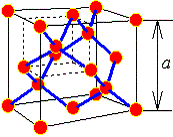
\includegraphics[width=0.8\textwidth]{硅晶体.png}
        \caption{硅晶体}
      \end{figure}
    \end{column}
  \end{columns}

\end{frame}

\begin{frame}
  \frametitle{间隙式扩散(interstitial)}

  \begin{columns}
    \begin{column}{0.7\textwidth}
      间隙式扩散是指原子在材料的晶格间隙中移动的现象。这种扩散方式的特点是扩散原子较小,可以穿过较大的基体原子之间的间隙。相比于置换式扩散,间隙式扩散更为迅速,因为间隙原子需要克服的势垒较低,并且其扩散路径较短。
    \end{column}
    \begin{column}{0.3\textwidth}
      \begin{figure}
        \centering
        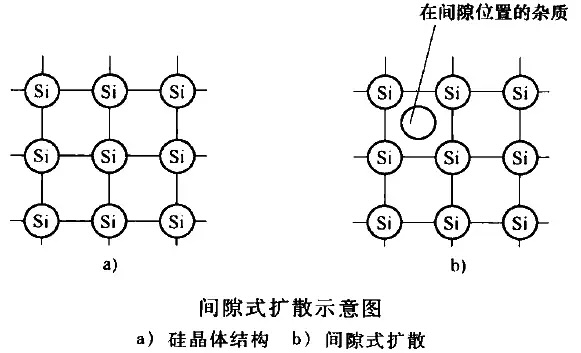
\includegraphics[width=0.8\textwidth]{间隙式扩散示意图.jpeg}
        \caption{间隙式扩散示意图}
      \end{figure}
    \end{column}
  \end{columns}

\end{frame}

\begin{frame}
  \frametitle{间隙式扩散(interstitial)}

  \begin{block}{间隙扩散杂质}
    Au,Fe,Cu,Ni,Zn,Mg
  \end{block}

  \begin{columns}
    \begin{column}{0.7\textwidth}
      \begin{itemize}
        \item 间隙原子在移动过程中需要克服的能量障碍称为\textbf{势垒高度 $E_i$} , $E_i$ 约为 0.6 ~ 1.2 eV
        \item 跳跃几率和温度有关,这是因为温度影响\textbf{原子的热振动能量}。
          跳跃几率可以用以下公式表示:
          \[
            P_i = v_0 \exp(-\frac{E_i}{kT})
          \]
          $v_0 = 10^{13} \to 10^{14}/s$:振动频率,间隙原子在晶格中振动的频率。
        \item 快扩散杂质:具有较高的扩散速率
      \end{itemize}
    \end{column}
    \begin{column}{0.3\textwidth}
      \begin{figure}
        \centering
        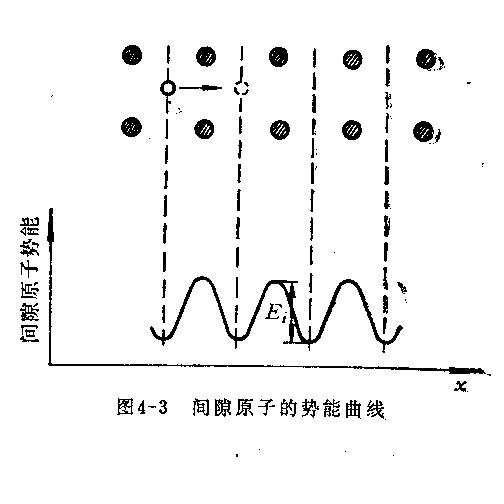
\includegraphics[width=0.8\textwidth]{间隙原子的势能曲线.png}
        \caption{间隙原子的势能曲线}
      \end{figure}
    \end{column}
  \end{columns}

\end{frame}

\begin{frame}
  \frametitle{ 跳跃几率(Jump Frequency)}

\textbf{跳跃几率}是指在扩散过程中,一个原子从一个位置跳跃到相邻位置的概率。这是一个统计量,表示在单位时间内,原子移动到邻近位置的频率。跳跃几率在理解和描述原子扩散行为中具有重要意义,尤其在半导体、金属和合金的扩散过程中。

跳跃几率的关键因素

\begin{itemize}
  \item \textbf{势垒高度(Activation Energy, \( E \))}:原子在扩散过程中需要克服的能量障碍,越高的势垒意味着越低的跳跃几率。
  \item \textbf{温度(Temperature, \( T \))}:温度越高,原子获得的热能越多,越容易克服势垒。
  \item \textbf{振动频率(Vibrational Frequency, \( \nu_0 \))}:原子在晶格中振动的频率。
\end{itemize}
\end{frame}

\begin{frame}
  \frametitle{跳跃几率的公式}

  跳跃几率通常用以下公式表示:
  \[ P = \nu_0 \exp\left(-\frac{E}{kT}\right) \]

其中:

\begin{itemize}
  \item \( P \) 是跳跃几率。
  \item \( \nu_0 \) 是振动频率,通常在 \( 10^{13} \sim 10^{14} \) Hz 之间。
  \item \( E \) 是原子需要克服的势垒高度(激活能)。
  \item \( k \) 是玻尔兹曼常数,约为 \( 1.38 \times 10^{-23} \) J/K。
  \item \( T \) 是绝对温度(开尔文)。
\end{itemize}
\end{frame}

\begin{frame}
  \frametitle{跳跃几率的公式解析}

\begin{itemize}
  \item 指数项 \(\exp\left(-\frac{E}{kT}\right)\):该项描述了原子克服势垒的概率。随着温度 \( T \) 的升高或势垒 \( E \) 的降低,这个概率增大。
  \item 振动频率 \(\nu_0\):反映了原子在晶格中振动的频率,代表了原子在每一单位时间内尝试跳跃的次数。
\end{itemize}

\textbf{半导体中的跳跃几率的实际应用}

在半导体材料中,掺杂原子的扩散行为很大程度上由跳跃几率决定。通过控制温度和了解激活能,可以预测和控制掺杂原子的扩散行为,从而优化半导体器件的性能。
\end{frame}

\begin{frame}
  \frametitle{替位式扩散(substitutional)}

  \begin{columns}
    \begin{column}{0.7\textwidth}
      替位扩散是指杂质原子占据晶体中正常原子的位置并通过晶体移动的过程。此种扩散方式主要依赖于晶体中的空位。

      替位原子的运动机制
    
      替位原子的运动需要相邻位置有空位(vacancy),原子通过空位的交换移动到新的位置。替位式扩散通常较为缓慢,因为在固体中形成空位需要较高的能量。
    
      对于某些元素如B(硼)和P(磷),其替位式扩散实际情况更复杂,包含了硅自间隙原子的作用,这种扩散机制称为填隙式或推填式扩散。(见后)
    \end{column}
    \begin{column}{0.3\textwidth}
      \begin{figure}
        \centering
        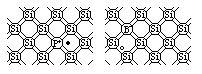
\includegraphics[width=0.8\textwidth]{Si中的V族杂质和III族杂质.png}
        \caption{Si中的V族杂质和III族杂质}
      \end{figure}
    \end{column}
  \end{columns}

\end{frame}

\begin{frame}
  \frametitle{替位式扩散(substitutional)}

  \begin{block}{替位扩散杂质}
    Al,Ga,In,B,P,As,Sb
  \end{block}

  \begin{columns}
    \begin{column}{0.7\textwidth}
      \begin{itemize}
        \item 替位原子必须越过的势垒高度 $E_s$ , $E_s$ 约为 3.0 ~ 4.0 eV
        \item 空位浓度公式
          \[
            N_v = N \exp(-\frac{E_{vac}}{kT})
          \]
          其中 $E_{vac}$ 为空位形成能量,$N$ 为晶格原子数,$T$ 为绝对温度,$k$ 为玻尔兹曼常数
      \end{itemize}
    \end{column}
    \begin{column}{0.3\textwidth}
      \begin{figure}
        \centering
        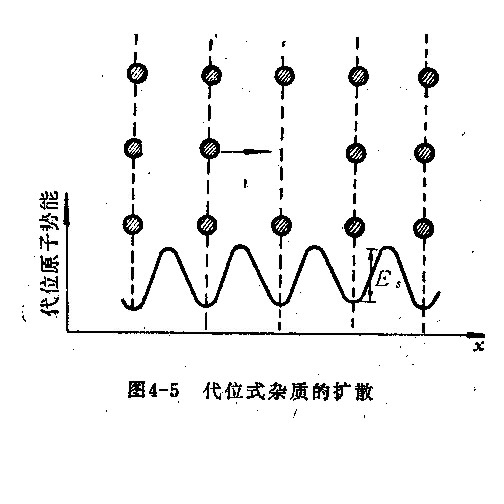
\includegraphics[width=0.8\textwidth]{代位原子的势能曲线.png}
        \caption{代位原子的势能曲线}
      \end{figure}
    \end{column}
  \end{columns}

\end{frame}

\begin{frame}
  \frametitle{替位式扩散(substitutional)}

  替位扩散杂质 Al,Ga,In,B,P,As,Sb

  \begin{columns}
    \begin{column}{0.7\textwidth}
      \begin{itemize}
        \item 跳跃几率和温度有关,跳跃几率
          \[
            P_v = v_0 \exp(-\frac{E_s}{kT})
          \]
        \item 振动频率 $v_0 = 10^{13} \to 10^{14}/s$
        \item 慢扩散杂质:替位扩散通常比间隙扩散慢,因为形成空位需要较高的能量,且替位原子在晶体中移动时需要克服较高的能量势垒。
      \end{itemize}
    \end{column}
    \begin{column}{0.3\textwidth}
      \begin{figure}
        \centering
        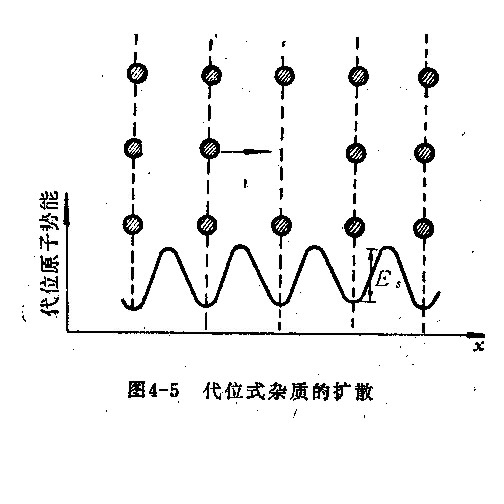
\includegraphics[width=0.8\textwidth]{代位原子的势能曲线.png}
        \caption{代位原子的势能曲线}
      \end{figure}
    \end{column}
  \end{columns}

\end{frame}

\begin{frame}
  \frametitle{推填式扩散}

  填隙式(interstitial assisted kick-out)或推填式扩散(Interstitialcy-assited)
  \begin{columns}
    \begin{column}{0.7\textwidth}
      填隙式扩散是一个两步过程,涉及间隙原子和替位原子的相互作用:

      间隙原子移动:掺杂原子首先进入晶格的间隙位置,成为间隙原子。
      间隙原子推挤基体原子:间隙原子推动或“踢出”一个基体原子,使其变成间隙原子,而原来的间隙原子则占据了被踢出的基体原子的位置。这一步导致原来的间隙原子转变为替位原子。
      这种机制有效地结合了间隙扩散和替位扩散的特点,使得某些掺杂元素能够更有效地在晶格中扩散。
    \end{column}
    \begin{column}{0.3\textwidth}
      \begin{figure}
        \centering
        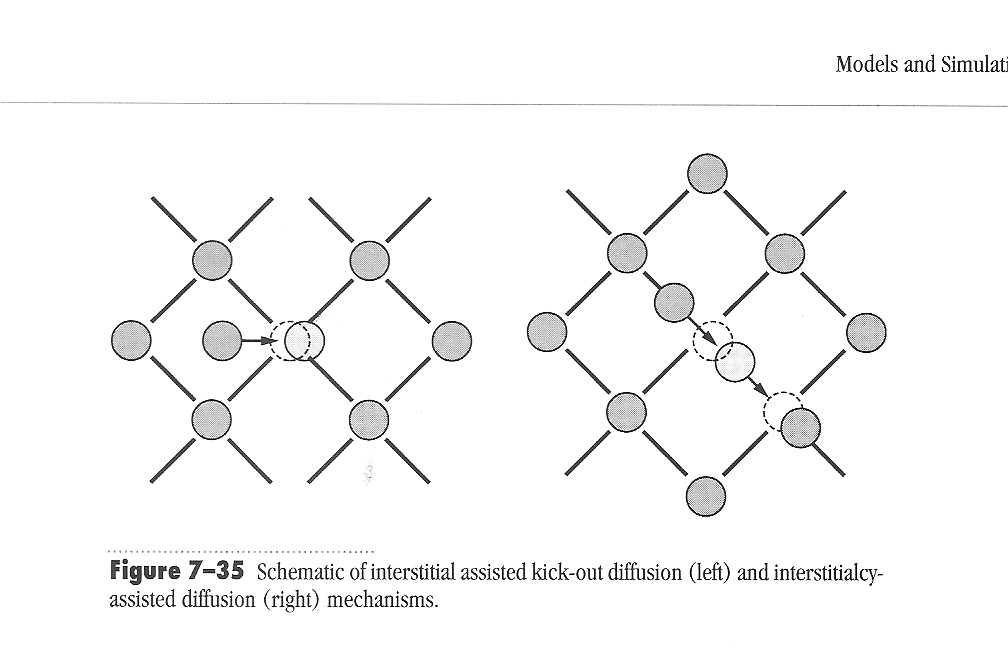
\includegraphics[width=0.8\textwidth]{填隙式扩散.png}
        \caption{填隙式扩散}
      \end{figure}
    \end{column}
  \end{columns}

\end{frame}

\begin{frame}
  \frametitle{本征扩散}

  \begin{block}{本征掺杂(Intrinsic Doping)}
    当掺杂浓度 \( N_A \)(受主浓度)和 \( N_D \)(施主浓度)都小于固有载流子浓度 \( n_i \) 时,半导体处于本征状态,即本征掺杂。这种情况下,半导体的导电性主要由本征载流子(电子和空穴)决定。
  \end{block}
\end{frame}

\begin{frame}
  \frametitle{本征扩散系数}

  本征扩散系数 \( D_i \) 表示在本征掺杂条件下,杂质原子在半导体中的扩散行为。其表达式为:
  \[ D_i = D^{0} \exp\left(-\frac{E_a}{kT}\right) \]

  其中:
  \begin{itemize}
    \item \( D_i \) 是本征扩散系数。
    \item \( D^0 \) 是预因子(pre-exponential factor),主要由晶格的几何尺寸和振动频率 \( v_0 \) 决定,且与温度弱相关。
    \item \( E_a \) 是本征扩散的激活能。
  \end{itemize}

\end{frame}

\begin{frame}
  \frametitle{本征扩散系数}
  
  \begin{columns}
    \begin{column}{0.7\textwidth}
      \begin{block}{表观扩散系数}
        表观扩散系数 \( D^0 \) 可以通过以下公式表示:
        \[ D^0 = a^2 v_0 \]
        
        其中:
        \begin{itemize}
          \item \( a \) 是晶格常数,表示晶格的几何尺寸。
          \item \( v_0 \) 是振动频率,通常在 \( 10^{13} \sim 10^{14} \) Hz 之间。
          \item 单位为 \( \mathrm{cm^2/s} \),表示扩散系数的尺度。
        \end{itemize}
      \end{block}
    \end{column}
    \begin{column}{0.3\textwidth}
      \begin{figure}
        \centering
        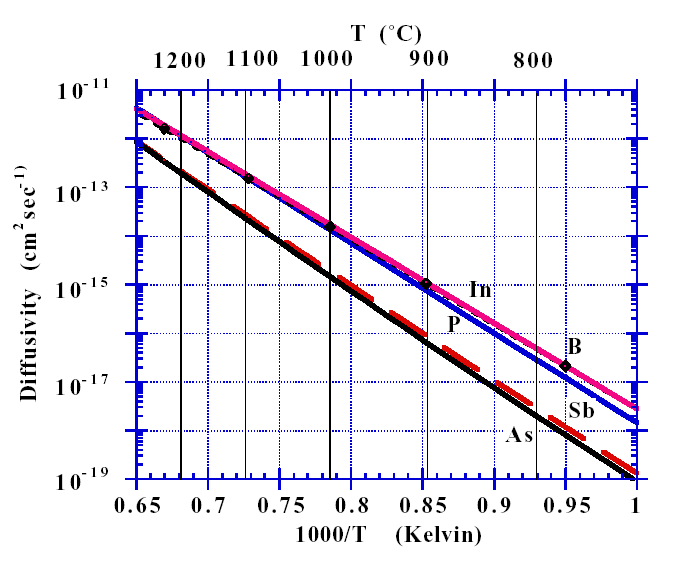
\includegraphics[width=0.8\textwidth]{本征扩散系数因子和激活能.png}
        \caption{本征扩散系数因子和激活能}
      \end{figure}
    \end{column}
  \end{columns}



\end{frame}
    
\begin{frame}
  \frametitle{半导体工艺中的本征扩散系数}
    
  在半导体制造工艺中,不同掺杂原子(如磷、砷、硼等)在单晶硅中的扩散行为各不相同。了解这些掺杂原子的本征扩散系数因子和激活能对优化掺杂工艺至关重要。
    
    砷(As)的优势
    
    \begin{itemize}
      \item 小扩散系数(Small \( D \)):砷在硅中的扩散系数较小,意味着扩散过程更容易控制,掺杂分布更精确。
      \item 大固溶度(High Solubility):砷在硅中的固溶度较大,可以实现较高的掺杂浓度,从而调节半导体材料的电学特性。
    \end{itemize}

    本征扩散系数和表观扩散系数的理解对于半导体掺杂工艺的优化至关重要。通过调整温度和选择合适的掺杂原子,可以控制掺杂分布和浓度,进而影响半导体器件的性能。砷作为掺杂原子的优势在于其小扩散系数和大固溶度,使其在精确掺杂和高浓度掺杂中具有优越性。
\end{frame}

\makebottom

\end{document}
